Serial Parrallel Interface (SPI) er en måde at lave hurtig seriel dataudveksling på. SPI er udviklet af Motorola og fungerer ved at man
har, som regel, en enkelt master enhed der styrer flere slave enheder. Ved SPI er der er ingen fejl-check men adressering af flere ender kan dog være 
HW krævende. I EasyWater8000 projektet er der SPI kommunikation imellem Master(devkit8000)
og Enhed(PSoC), det giver muligheden for at overføre flere data på samme tid imellem disse to.

\begin{figure}[H] \centering
{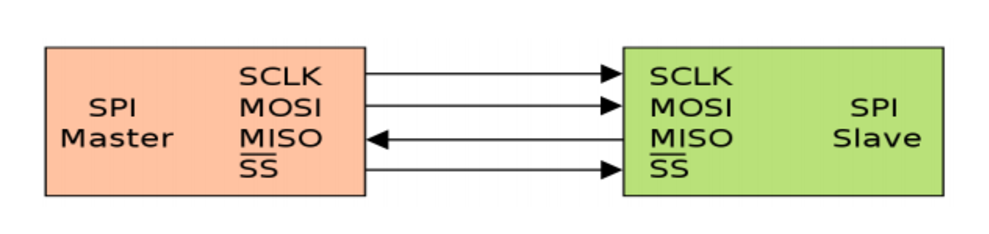
\includegraphics[width=\textwidth]{filer/design/Billeder/SPI_MASTER_SLAVE}}
\caption{SPI}
\label{lab:SPI}
\raggedright
\end{figure}

På figur \ref{lab:SPI} ses en typisk opkobling imellem Master og Slave, det kræver 4 tråde.
\begin{itemize}
 	\item SS står for "Slave select".
 	\item MISO står for "Master in slave out".
 	\item MOSI står for "Master out slave in". 
	\item SCLK står for "Serial clock" 
\end{itemize}

SPI kommunikation er baseret på skifteregister princippet, som ses på figur \ref{lab:SPI_REGISTER}. Der vælges hvilken slave der 
ønskes at skrives til ved slave select(SS), derefter shiftes et 8-bit register 1 bit ad gangen. Serial clock er den clock der sørger for at
shiftningen af bits sker korrekt, clockfrekvensen må ikke overstige grænsen for hvad enhederne kan håndtere.

\begin{figure}[H] \centering
{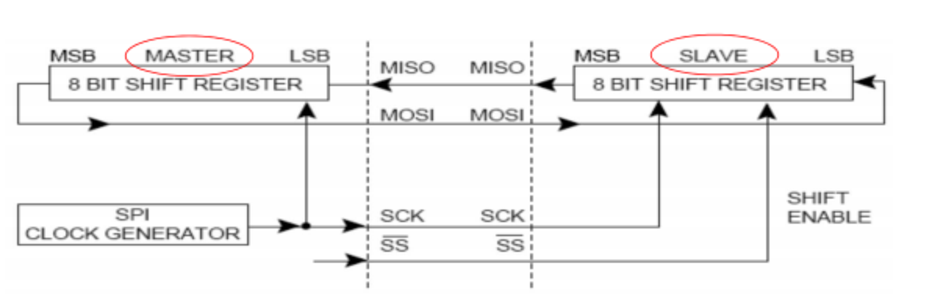
\includegraphics[width=\textwidth]{filer/design/Billeder/SPI_REGISTER}}
\caption{SPI register}
\label{lab:SPI_REGISTER}
\raggedright
\end{figure}  

En oftes anvendt kommunikation mellem master og slave foregår ved at master sætter SS til 0. Den fortæller nu til slaven at den er klar til 
dataoverførelse. Nu sender masteren en bit over til slaven og påbegynder en full duplex data transmission, samtidigt sender slaven en bit over
til masteren. Denne process fortsætter indtil masteren har sendt alle sine bits, derefter stopper masteren med at toggle på clocken og slave 
enheder bliver frigivet.

\subsection{Driver}

I SPI-kommunikationen er der taget udgangspunkt i HAL Exercise 7 \footnote{Hardware abstraktioner. Exercise 7: LDD with SPI. Øvelse med SPI Kommunikation}, der er dog lavet kraftigt om i kernemodul og driver. Så de tilpasses EasyWater8000s behov.

Driveren opbygges med en Skrive og en Læse metode, der begge kan læse eller skrive én 8 bits karakter(char).

\subsubsection*{Pseudokode}

\begin{lstlisting}[language=C]
int write(data){
Send data parameter ud paa SPI netvaerket
}
int read(*datapointer){
Modtag data
Flyt data til datapointer parameter
}
\end{lstlisting}